\documentclass[11pt]{article}

\usepackage[a4paper, total={6in, 8in}]{geometry}
\usepackage{graphicx}
\usepackage{multicol}
\usepackage{multirow}

\title{July2023 CSE300 Week9 Online Evaluation}
\author{2005076}
\date{\today}

\begin{document}
    \maketitle
    \tableofcontents
    \pagebreak

    \section{RISC Architecture}
    \begin{figure}[h]
        \centering
        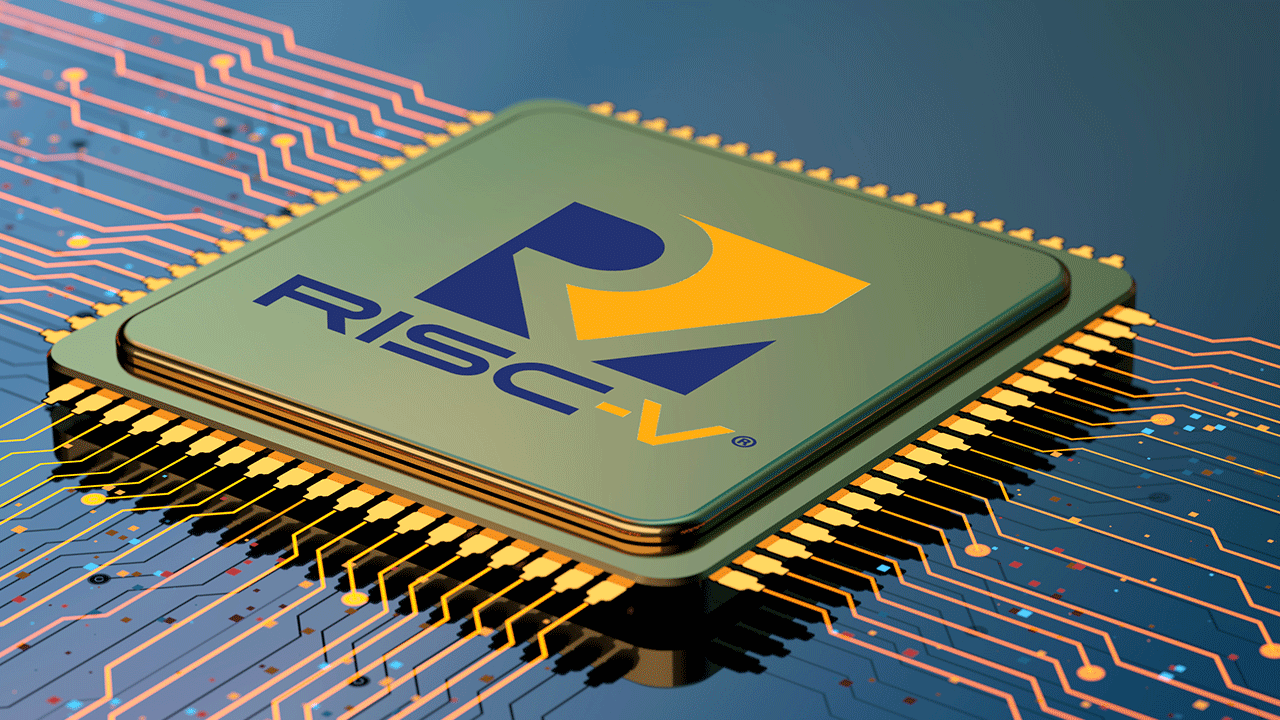
\includegraphics[scale = 0.25]{Images/risc.png}
        \caption{RISC Architecture}
        \label{fig:enter-label}
    \end{figure}

    \section{Tables in \LaTeX}
    \begin{table}[h]
        \centering
        \begin{tabular}{|c|c|c|c|}
            \hline
            \multirow{10}{*}{numeric literals} & \multirow{5}{*}{integers} & in decimal & 8743 \\
            \cline{3-4}
            & & \multirow{2}{*}{in octal} & Oo7464 \\
            \cline{4-4}
            & & & 00103 \\
            \cline{3-4}
            & & \multirow{2}{*}{in hexadecimal} & 0x5A0FF \\
            \cline{4-4}
            & & & 0xE0F2 \\
            \cline{2-4}
            & \multirow{5}{*}{fractionals} & \multirow{5}{*}{fractionals} & 140.58\\
            \cline{4-4}
            & & & 8.04e7\\
            \cline{4-4}
            & & & 0.34\\
            \cline{4-4}
            & & & 5.74\\
            \cline{4-4}
             & & & 47e22\\
            
            \hline
        \end{tabular}
        \caption{A table in \LaTeX}
        \label{tab:my_label}
    \end{table}

    Table 1 shows a table that contains cells spanning multiple columns and multiple rows. \cite{2nd}

    \pagebreak
    \section{Writing Equations in Latex}
    \begin{equation}[h]
        L_{split} = \frac{1}{2}\left[ \frac{G_L^2}{H_L+\lambda} +  \frac{G_R^2}{H_R+\lambda} -  \frac{(G_L+G_R)^2}{H_L+ H_R+\lambda} \right] - \gamma
    \end{equation}

    Equation 1 has been displayed above.\cite{ML}

    \section*{Untitled Section}
    You need to display this section in your output PDF file. This section contains information
    that may help you prepare the bibliography section. By the way, this section \textbf{will not show up} in the table of contents.

    \begin{enumerate}
        \item  Citation about the Greedy Forest Article
        \begin{itemize}
            \item \textbf{ Authors:} T. Zhang, R. Johnson
            \item \textbf{ Title:}  Learning nonlinear functions using regularized greedy forest
            \item \textbf{ Year:} 2014
            \item \textbf{ Journal:}  IEEE Transactions on Pattern Analysis and Machine Intelligence
            
        \end{itemize}
        \item Citation about the Random Forest Article
        \begin{itemize}
            \item \textbf{ Authors:}  L. Breiman
            \item \textbf{ Title:}  Random Forests
            \item \textbf{ Journal:}   Machine Learning
            \item \textbf{ Year:} 2001
        \end{itemize}
    \end{enumerate}

    \bibliographystyle{plain}
    \bibliography{ref}
    
\end{document}